%!TEX root = ..\lections.tex

Сверхпроводимость -- это свойство некоторых материалов обладать 
нулевым электрическим сопротивлением, когда их температура достигает 
значания ниже некоторого критического. Такое свойство демонстрируют несколько десятков чистых элементов, керамик и сплавов.

Рассмотрим систему, состоящую из двух сверхпроводников, разделенных 
тонким (толщина порядка $10^{-7}$ см) изолирующим слоем, образованным, например, нормальным металлом. В 1962 г. 22-х летний студент-дипломник 
Б.Джозефсон (Brian Josephson) опубликовал статью, в которой, опираясь на
экспериментальные результаты Гиавера, пришел к выводу о том, что через
такой контакт возможно протекание сверхпроводящих токов. В частности,
протекание постоянного тока даже в случае отсутствия разности потенциалов
между сверхпроводниками. С точки зрения классических представлений такой
эффект невозможен. Джозефсон показал, что протекание сверхпроводящих
токов является следствием туннелирования так называемых куперовских пар
через контакт. Куперовская пара представляет собой квазичастицу,
образованную за счет взаимодействия и связывания двух электронов в
сверхпроводнике. Поток куперовских пар и формирует ток при
сверхпроводимости. Состояние куперовской пары можно описать с помощью
волновой функции. Оказывается, что в сверхпроводнике куперовские пары не
могут двигаться независимо друг от друга. Взаимодействие таких пар приводит
к их взаимной упорядоченности, в следствие которой состояние куперовских
пар в сверхпроводнике характеризуется \textbf{единой волновой функцией}. Другими
словами, куперовские пары скапливаются в одном и том же квантовом
состоянии и поэтому описываются одной и той же волновой функцией.
\section{Стационарный и нестационарный эффекты}%
\label{sec:11.1}

Предположим, что волновые функции куперовских пар в
сверхпроводниках не зависят от пространственных координат и изменяются
только во времени. В таком приближении волновые функции задаются
следующим образом
\begin{equation}
        \label{eq:11.1}
        \Psi_i = \sqrt{\rho_{i}} e^{i\phi_i},~ i =1,2,
\end{equation}
где $\rho_i$ -- плотность зарядов электронов в сверхпроводниках, а $\phi_i$ -- общая для всех частиц фаза в $i$-ом сверхпроводнике. При достаточном сближении сверхпроводников их волновые функции начинают перекрываться в области
изолирующего зазора (барьера), формируя туннельный контакт. Возникает процесс переноса куперовских пар
через барьер, который описывается следующей системой для волновых функций
\begin{equation}
        \label{eq:11.2}
        \begin{cases}
                i \hbar \pdv{\Psi_1}{t} = E_1 \Psi_1 + K \Psi_2,\\
                i \hbar \pdv{\Psi_2}{t} = E_2 \Psi_2+ K \Psi_1,
        \end{cases}
\end{equation}
где $\hbar$-- постоянная Планка, $E_1$, $E_2$ -- энергии основных состояний каждого из проводников, $K$ - амплитуда взаимодействия двух состояний контакта, зависящая от его специфики (геометрии электродов, параметров барьера и др.). Приложим к контакту постоянную разность потенциалов $V$, которая приведет к сдвигу
\begin{equation}
        \label{eq:11.3}
        E_1-E_2=2eV.
\end{equation}
Без ограничения общности будем считать, что энергия отсчитывается от среднего между величинами $E_1$ и $E_2$. Тогда \eqref{eq:11.2} и \eqref{eq:11.3} имеем
\begin{equation}
        \label{eq:11.4}
        \begin{cases}
                i \hbar \pdv{\Psi_1}{t} = eV\Psi_1+ K\Psi_2,\\
                i \hbar \pdv{\Psi_2}{t} = - eV \Psi_2 + K \Psi_1.
        \end{cases}
\end{equation}
Подставляя в \eqref{eq:11.4} выражения $\Psi_1$ и $\Psi_2$ из \eqref{eq:11.1} и разделяя в полученных
уравнениях действительные и мнимые части, находим
\begin{equation}
        \label{eq:11.5}
        \pdv{\rho_1}{t} = \frac{2K \sqrt{\rho_1\rho_2}}{\hbar} \sin \phi, \quad
        \pdv{\rho_2}{t} - \frac{2K \sqrt{\rho_1 \rho_2}}{\hbar} \sin \phi,
\end{equation}
\begin{align}
        \label{eq:11.6}
        \pdv[]{\phi_{1}}{t} = -\frac{eV}{\hbar} - \frac{K}{\hbar}\sqrt{\frac{\rho_{2}}{\rho_{1}}}
        \cos \phi, \\
        \pdv[]{\phi_{2}}{t} = -\frac{eV}{\hbar} - \frac{K}{\hbar}\sqrt{\frac{\rho_{1}}{\rho_{2}}}
        \cos \phi, \\
\end{align}
где $\phi = \phi_{2}-\phi_{1}$. Обозначим через $I_s$ ток куперовских пар, так называемый
сверхток, который задается через $\rho_{1}$ и $\rho_{2}$ следующим образом
\begin{equation}
        \label{eq:11.7}
        I_s = \pdv[]{\rho_{1}}{t}= - \pdv[]{\rho_{2}}{t}.
\end{equation}
Принимая во внимание \eqref{eq:11.7}, получаем из \eqref{eq:11.6}, что
\begin{equation}
        \label{eq:11.8}
        I_s = \frac{2K}{\hbar}\sqrt{\rho_{1}\rho_{2}} \sin \phi.
\end{equation}
Включим контакт во внешнюю цепь с истояником постоянного тока $I>0$. За счет действия этого источника
значения величин $\rho_{1}$ и $\rho_{2}$ могут поддерживаться постоянными, поскольку он непрерывно компенсирует потери куперовских пар уже протуннелированных через барьер. Предположим для простоты,
что $\rho_{1}= \rho_{2}=\rho= \const$. Тогда из \eqref{eq:11.8} имеем
\begin{equation}
        \label{eq:11.9}
        I= I_{max}\cdot \sin\phi,
\end{equation}
где $I_{max} = \frac{2K}{\hbar}\rho$. Из \eqref{eq:11.9} следует, что при $I<I_{max}$ существует
разность фаз $\phi$, при которой через контакт будет протекать постоянный ток. 
Заметим, что в \eqref{eq:11.9} никак не входит напряжение на контакте. Постоянный ток через контакт протекает при нулевой разности потециалов!
Этот эффект называют \textbf{стационарным эффектов Джозефсона.}. Он был подтвержден экспериментально
Андерсоном и Роуэлом через год после теоретической работы Джозефсона.

Рассмотрим теперь систему \eqref{eq:11.6} для фаз волновых функций. При сделанных выше предположениях
из \eqref{eq:11.6} следует, что
\begin{equation}
        \label{eq:11.10}
        \dv[]{\phi}{t}= \frac{2eV}{\hbar}.
\end{equation}
Уравнение \eqref{eq:11.10} описывает ещё один удивительный эффект, предсказанный Джозефсоном. 
При постоянном напряжении на контакте через него протекает высокочастотный переменный ток.
Это явление называют \textbf{нестационарным эффектом Джохевсона}. Заметим,
что частота переменного тока пропорциональна величине приложенного напряжения. Однако, даже при очень малых напряжениях эта частота, оказывается , может лежать в очень широких пределах. 
Например, для некоторых сверхпроводников при напряжении $V=1 \text{ мВ }$ достигнута генерация переменного тока с частотой $4.85\cdot 10^{11}$ Гц.

\section{Эквивалентная схема контакта}%
\label{sec:11.2}

Кроме сверх тока, задаваемого выражением \eqref{eq:11.9}, через Джозевсоновский контакт протекает и обычный (нормальный) ток, вызванный туннелированием отдельных электронов. Контакт обладает также 
и емкостными свойствами, связанными со специфической конфигурацией контакта. Принимая эти
свойства во внимание, получим электрическую схему контакта, представленную на рис.\ref{fig:11.1}.
\begin{figure}[h]
        \centering
        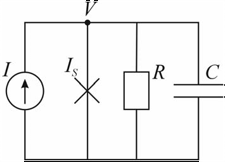
\includegraphics[width=0.4\linewidth]{fig/lect11/1}
        \caption{Эквивалентная электрическая схема Джозефсоновского контакта.}
        \label{fig:11.1}
\end{figure}
Запишем закон Кирхгофа для полного тока через контакт
\begin{equation}
        \label{eq:11.11}
        C \dv[]{V}{t} + \frac{V}{R } + I_{max} \sin \phi = I.
\end{equation}
Исключая в \eqref{eq:11.11}, с помощью соотношения \eqref{eq:11.10}, переменную $V$, получим
следующее уравнение
\begin{equation}
        \label{eq:11.12}
        \frac{\hbar C}{2e} \dv[2]{\phi}{t} + \frac{\hbar}{2eR}\dv{\phi}{t}+I_{max}\sin \phi =I.
\end{equation}
Введем в \eqref{eq:11.12} новое время и параметры
\begin{equation}
        \label{eq:11.13}
        \ddot \phi + \lambda \ddot \phi + \sin \phi = \gamma,
\end{equation}
где точкой обозначено дифференцирование по времени $\tau$.

Заметим, что уравнение \eqref{eq:11.13} описывает также динамику совершенно далеких от теории
сверхпроводимости физических систем -- механического маятника в вязкой (параметр $\lambda$) среде, 
находящегося под действием постоянного внешнего момента $\gamma$ (см. лекцию \ref{lect8}),  
и системы фазовой автоподстройки частоты (ФАПЧ), содержащую в цепи управления линейный фильтр, постоянную времени которого характеризует параметр $\lambda$ (см. лекцию \ref{lect4}).
В случае маятника переменная $\phi$-- угол отклонения от равновесия, а в случае системы ФАПЧ -- 
разность фаз между двух генераторов, имеющих начальную расстройку по частоте $\gamma$. Поэтому 
полученные ниже результаты исследования динамики уравнения \eqref{eq:11.13} можно использовать для понимания поведения и этих физических объектов. 

\section{Динамика модели}%
\label{sec:11.3}

Перепишем уравнение \eqref{eq:11.13} в виде эквивалентной системы 
\begin{equation}
        \label{eq:11.14}
        \begin{cases}
                \dot \phi = y,\\
                \dot y = \gamma - \sin \phi - \lambda y.
        \end{cases}
\end{equation}
Будем рассматривать систему \eqref{eq:11.14} в области параметров 
$D= \qty{\lambda, \gamma| \gamma \geq 0, \lambda\geq 0}.$ Система \eqref{eq:11.14} имеет цилиндрическое
фазовое пространство $G= S^{1} \times \R,$ поскольку её правая часть $2\pi$-периодична по переменной $\phi$.

\subsection{Консервативный случай}%
\label{sub:11.3.1}

При $\lambda=0$ система \eqref{eq:11.14} принимает форму нелинейного консервативного осциллятора, полная энергия которого сохраняется и задается следующим образом
\begin{equation}
        \label{eq:11.15}
        E= E_{K}+ E_{\text{П}}=\const,
        E_{\text{П}}
\end{equation}
где 
\begin{equation}
        \label{eq:}
        E_{K}=\frac{y^2}{2}, \quad E_{\text{П}} = \int\limits_{\phi_{0}}^{\phi} \qty(\sin \xi -\gamma) \dd{\xi}, 
\end{equation}
где $\phi_{0}$ задает уровень, относительно которого отсчитывается потенциальная энергия.
Из соображений удобства построения графика функции $E_{\text{П}}(\phi)$, необходимого в дальнейшем,
выберем $\phi_{0}$ следующим образом
\begin{equation}
        \label{eq:}
        \phi_{0} =
        \begin{cases}
                \arcsin \gamma, \text{ если } \gamma\leq{1} \\
                \frac{\pi}{2}, \text{ если } \gamma> 1
        \end{cases}
\end{equation}
Для построения фазовых портретов осциллятора воспользуемся стандартной процедурой (см. лекцию \ref{lect5}), основанной на свойствах функции $E_{\text{П}}(\phi)$. На рис.\ref{fig:11.2} представлен
качественный вид функции $E_{\text{П}}(\phi)$ и соответствующие фазовые портреты для различных
значений параметра $\gamma$.

Заметим, что рассматриваемый осциллятор имеет на одном периоде <<угловой>> переменной $\phi$ два
состояния равновесия при $\gamma<1$, одно из которых седло, а другое -- центр, при $\gamma=1$ --
одно состояние равновесия с двумя нулевыми характеристическими показателями. При $\gamma>1$ 
состояний равновесия нет.

\begin{figure}[h]
        \centering
        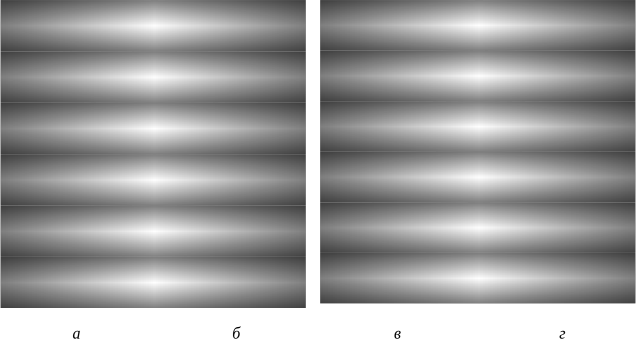
\includegraphics[width=\linewidth]{fig/lect11/2}
        \caption{Качественный вид функции $E_{\text{П}}(\phi)$ и соответствующие фазовые портреты
        для различных значений параметра $\gamma:$ 
$\gamma=0$ (a); $\gamma \in (0,1) ~ (b)$; $\gamma=1 ~ (c)$;  $\gamma>1~ (d).$}
        \label{fig:11.2}
\end{figure}

\subsection{Диссипативный случай}%
\label{sub:11.3.2}

Исследование системы \eqref{eq:11.4} при $\lambda>0$ начнем с установления важного свойства, связанного с её диссипативностью.

\subsubsection{Поглощающая область}%
\label{ssub:11.3.2a}

Непосредственно из системы \eqref{eq:11.4} имеет
\begin{equation}
        \label{eq:11.16}
        \dot y = \gamma - \sin \phi - \lambda y \leq \gamma+1 - \lambda y.
\end{equation}
Из \eqref{eq:11.6} следует, что $\dot y <0$ при любых значениях переменной $\phi \in S^1$,
если $y > \frac{1+\gamma}{\lambda}$. Следовательно, любая траектория системы \eqref{eq:11.14} 
с начальными условиями $\phi(0) \in S^1, ~ y(0) > \frac{1+\gamma}{\lambda}$ с течением времени приходит
в область на фазовом цилиндре $G$, расположенную при $y< \frac{1+\gamma}{\lambda}$. При этом, для 
$y> \frac{1+\gamma}{\lambda}$ переменная $y$ монотонно убывает вдоль любой траектории.
Аналогично,
\begin{equation}
        \label{eq:11.17}
 \dot y = \gamma - \sin \phi - \lambda y \geq \gamma - 1 - \lambda y.       
\end{equation}
В силу \eqref{eq:11.17} имеем
\begin{equation}
        \label{eq:}
        \dot y > 0, \text{ если } y< \frac{\gamma-1}{\lambda}.
\end{equation}
Отсюда следует, что любая траектория системы \eqref{eq:11.14} с 
начальными условиями $\phi(0) \in S^1,~y(0)< \frac{\gamma-1}{\lambda}$ с течением времени попадает в
область на фазовом цилиндре $G$, расположенную при $y>\frac{\gamma-1}{\lambda}$, а переменная $y$ 
при $y<\frac{\gamma-1}{\lambda}$ монотонно возрастает. Суммируя установленные выше свойства траектории 
системы \eqref{eq:11.14}, получаем, что область
\begin{equation}
        \label{eq:}
        G^{+} = \qty{ \phi,y\eval \phi \in S^{1}, \frac{\gamma-1}{\lambda}\leq y \leq \frac{\gamma+1}{\lambda} }
\end{equation}
притягивает все траектории этой системы с начальными условиями вне этой области.
Другими словами, $G^+$ -- поглощающая область (см. лекцию \ref{lect1}). 
Заметим, что границу области  $G^+$ траектории системы \eqref{eq:11.14}
пересекают в одну сторону -- снаружи внутрь. Поэтому траектории с начальными условиями из области
$G^+$ остаются в ней при любом $\tau>0$. Далее будем рассматривать систему \eqref{eq:11.14} 
в области $G^+$, содержащей все её неблуждающие траектории.

\subsubsection{Состояние равновесия и их локальные свойства}%
\label{ssub:11.3.2b}

Из \eqref{eq:11.4} следует, что координаты состояний равновесия определяются 
следующей системой
\begin{equation}
        \label{eq:11.18}
        y=0,~\gamma-\sin \phi - \lambda y =0.
\end{equation}
Решая систему \eqref{eq:11.18}, устанавливаем, что система \eqref{eq:11.14} имеет при 
$0 \leq \gamma <1$ два состояния равновесия -- $O_{1}(\phi=\phi_{1},y=0)$ и 
$O_{2}(\phi=\phi_{2},y=0)$, где $\phi_{1}=\arcsin \gamma,~ \phi_{2}= \pi-\arcsin \gamma $, при 
$\gamma=1$ - одно $O_{0}(\phi=\frac{\pi}{2},y=0)$, а при $\gamma>1$ состояний равновесия нет.
Несложно показать ( предлагаем читателю проделать это самостоятельно ) с помощью метода линеаризации
(см. лекцию \ref{lect4}), что состояние равновесия $O_{1}$ является асимптотически устойчивым,
а $O_{2}$ - седлом.
Состояние равновесия $O_{1}$-- устойчивый фокус, если $\lambda < 2 \qty(1-\gamma^2)^\frac{1}{4}$
и устойчивый узел в противоположном случае (см. рис.\ref{fig:11.3}а).

Найдем критические направления сепаратрис седла $O_{2}$. Для этого линеаризуем систему \eqref{eq:11.14}
в окрестности точки $O_{2}$.
\begin{figure}[h]
        \centering
        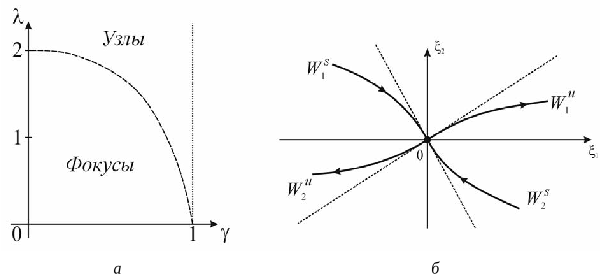
\includegraphics[width=\linewidth]{fig/lect11/3}
        \caption{Качественное разбиение плоскости параметров $D$ 
        на области, отвечающие различным типам состояния равновесия $O_{1}$ (a); качественное
представление критических направлений седла $O_{2}$ (b).}
        \label{fig:11.3}
\end{figure}
В результате получим линеаризованную систему следующего вида
\begin{equation}
        \label{eq:11.19}
        \begin{cases}
                \dot \xi_{1} = \xi_{2} \\
                \dot \xi_{2} = \sqrt{1 - \gamma^2} \xi_{1} - \lambda \xi_{2}
        \end{cases}
\end{equation}
Перепишем \eqref{eq:11.19} в виде одного эквивалентного уравнения
\begin{equation}
        \label{eq:11.20}
        \dv[]{\xi_{2}}{\xi_{1}} = \frac{ \sqrt{ 1 - \gamma^2} \xi_{1} - \lambda \xi_{2}}{\xi_{2}}.
\end{equation}
Как известно (см. лекцию \ref{lect4}), у линейных систем сепаратрисы седел представляют 
собой прямые. Поэтому будем искать уравнения сепаратрис седла системы \eqref{eq:11.19} в
виде
\begin{equation}
        \label{eq:11.21}
        \xi_{2}=k \xi_{1},
\end{equation}
где $k$-- коэффициент, который требуется найти.
Подставляя \eqref{eq:11.21} в \eqref{eq:11.20}, получим
\begin{equation}
        \label{eq:11.22}
        \dv[]{\xi_{2}}{\xi_{1}}\eval_{\xi_{2}=k\xi_{1}} = 
        \frac{\sqrt{1 - \gamma^2} \xi_{1} - \lambda k \xi_{1}}{k\xi_{1}}
        = \frac{\sqrt{1-\gamma^2} - \lambda k}{k}.
\end{equation}
С другой стороны, из \eqref{eq:11.21} следует, что
\begin{equation}
        \label{eq:11.23}
        \dv[]{\xi_{2}}{\xi_{1}} = k.
\end{equation}
Приравнивая теперь правые части \eqref{eq:11.22} и \eqref{eq:11.23}, получаем для
нахождения $k$ квадратное уравнение, корни которого и определяют искомые 
коэффициенты
\begin{equation}
        \label{eq:11.24}
        k_{1,2} = - \frac{\lambda}{2} \pm \sqrt{ \frac{\lambda_{2}}{4} + \sqrt{ 1 - \gamma^2}}.
\end{equation}
Поскольку $k_{1}$, а $k_{2}<0,$ то в силу первого уравнения системы \eqref{eq:11.14}
в точке $O_{2}$ неустойчивые сепаратрисы касаются прямой с наклоном $k_{1}$, а устойчивые --
с наклоном $k_{2}$. Неустойчивую сепаратрису, выходящую в область $\xi_{2}>0$, обозначим через
$W_{1}^u$, а в область $\xi_{2}<0$-- через $W_{2}^u$. Аналогично, устойчивую сепаратрису,
приближающуюся к точке $O_{2}$ со стороны $y>0$, обозначим через
$W_{1}^s$, а со стороны $\xi_{2}<0$-- через $W_{2}^s$ (см. рис.\ref{fig:11.3}b).

При $\gamma=1$ состояния равновесия $O_{1}$ и $O_{2}$ сливаются в точке $O_{0}$,
которая исчезает при $\gamma>1$. Точка $O_{0}$ -- седло-узел с устойчивой 
узловой областью и неустойчивой сепаратрисой (см. лекцию \ref{lect8}). Таким
образом, при  $\gamma=1$ происходит бифуркация коразмерности 1  -- образования 
седло-узла.

 
\subsubsection{Функция Ляпунова}%
\label{ssub:11.3.2c}

При $0\leq \gamma<1$ введем в рассмотрение функцию
\begin{equation}
        \label{eq:11.25}
        V( \phi,y) = \frac{y^2}{2} + \int\limits_{\phi_{1}}^{\phi} \qty( \sin \xi - \gamma) \dd{\xi}. 
\end{equation}
Найдем производную 
этой функции в силу системы \eqref{eq:11.14}
\begin{equation}
        \label{eq:11.26}
        \dot V = y \cdot \dot y + \qty( \sin \phi - \gamma) \dot \phi =
        y\qty(\gamma - \sin \phi - \lambda y) + (\sin \phi -\gamma)y = - \lambda y^2 \leq 0.
\end{equation}
Из \eqref{eq:11.26} следует, что вдоль траектории системы \eqref{eq:11.14} при увеличении времени
$\tau$ линии уровня $V(\phi,y) = C = \const$ убывают.
Заметим, что условие $\dot V \eval_{y=0}$ не нарушает этого свойства.
В точках пересечения линий уровня $V(\phi,y) = C$ с прямой $y=0$ траектории системы \eqref{eq:11.14},
хотя и касаются этих линий, но продолжают свое движение в сторону их 
убывания. Рассмотрим вид линий уровня функции $V(\phi,y)$ на фазовом цилиндре, который,
очевидно, зависит от параметра $\gamma$.

\paragraph{Пусть $\gamma=0$.}%

В этом случае линии уровня качественно





                
